\section{Sensores Internos}
	\subsection{Sensores de Posición}
\subsubsection{Lineales y Rotativos}
Los sensores de posición lineal incluyen:

\begin{itemize}
	\item \textbf{Encóder incremental}:Este tipo de sensor convierte el movimiento en una serie de pulsos eléctricos que indican cambios en la posición, pero no su valor absoluto. Requiere un punto de referencia para determinar la posición inicial y utiliza dos señales desfasadas (A y B) para detectar dirección y velocidad. Estos constan, en su forma más simple, de un
	disco transparente con una serie de marcas opacas colocadas radialmente y equidistantes entre sí; de un sistema de iluminación en el que la luz es colimada de forma correcta, y de un elemento fotorreceptor (Figura 1). El eje, cuya posición se quiere medir, va acoplado al disco transparente. Con esta disposición, a medida que el eje gire se irán generando pulsos en el receptor cada vez que la luz atraviese cada marca. Llevando una cuenta de estos pulsos será posible conocer la posición del eje.
	\begin{figure}[h]
		\centering
		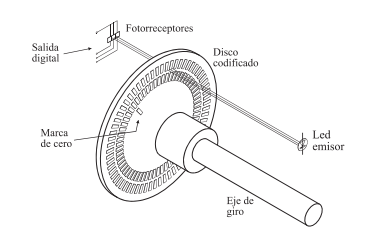
\includegraphics[width=0.8\textwidth]{img/encoderincremental.png}
		\caption{Disposición de un codificador óptico (encóder) incremental.}
		\label{fig:encoderincremental}
	\end{figure}
	
	
	\item \textbf{Encóder absoluto}:A diferencia del incremental, el encoder absoluto proporciona la posición exacta en todo momento, incluso después de un apagado. Funciona mediante un disco codificado con un patrón único para cada posición, permitiendo lecturas precisas sin necesidad de reiniciar.
	\begin{figure}[h]
		\centering
		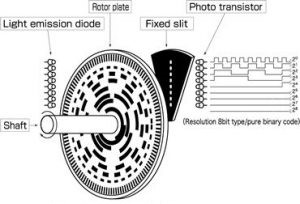
\includegraphics[width=0.6\textwidth]{img/encoderabsoluto.jpg}
		\caption{Estructura simplificada del encóder absoluto.}
		\label{fig:encoderabsoluto}
	\end{figure}
	
	
	\item \textbf{Potenciómetro}: Es un dispositivo de resistencia variable que expresa desplazamientos lineales o angulares en términos de voltaje, tal como se muestra en las figuras 3a) y b), respectivamente. Consiste en una clavija deslizante que hace contacto con un elemento resistivo; conforme se mueve este punto de contacto, la resistencia entre el contacto deslizante y las conexiones de los extremos del dispositivo cambia en proporción al desplazamiento, x y  para potenciómetros lineales y angulares, respectivamente.
	\begin{figure}[h]
		\centering
		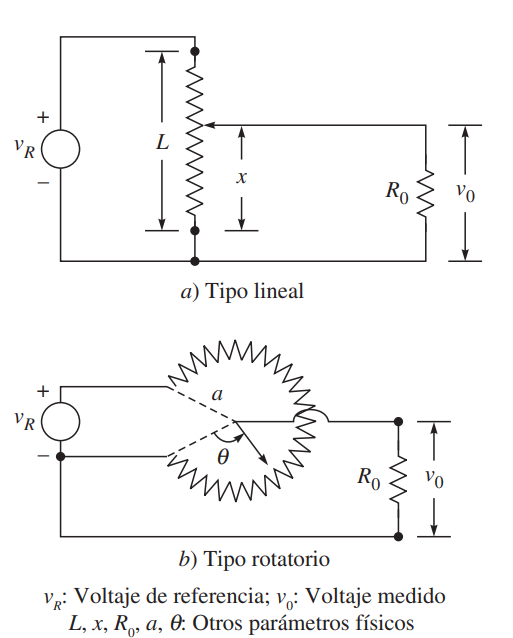
\includegraphics[width=0.4\textwidth]{img/potenciometro.png}
		\caption{Potenciómetros.}
		\label{fig:potenciometros}
	\end{figure}
	
	
	
	\item \textbf{LVDT}: El transformador diferencial lineal variable (LVDT) es un sensor de desplazamiento altamente preciso y confiable. Funciona con una señal de corriente alterna (CA), generando un voltaje proporcional al desplazamiento del núcleo móvil dentro de un campo magnético. Su estructura incluye un núcleo central rodeado por bobinas secundarias y una bobina primaria que crea el campo magnético. A medida que el núcleo se mueve, la señal de salida cambia de manera lineal con el desplazamiento. También existe el transformador diferencial rotativo (RVDT), que opera con el mismo principio pero para movimientos angulares. Su principio de funcionamiento es basado en la inducción electromagnética. En el esquema de la Figura 4, se observa un núcleo ferromagnético móvil que se desplaza dentro de un conjunto de bobinas:
	\item \textbf{Bobina primaria (Lp)}: Recibe una señal de excitación en corriente alterna (CA) y genera un campo magnético.
	\item \textbf{Bobinas secundarias (Ls1 y Ls2)}: Están ubicadas a ambos lados del núcleo y captan la variación del flujo magnético cuando el núcleo se mueve.
	\item \textbf{Núcleo móvil}: se mueve dentro de las bobinas y altera la relación de inductancias.
	
	El desplazamiento del núcleo altera la relación de inductancias entre las bobinas secundarias, modificando así la amplitud y fase de la señal de salida. Esto permite determinar la posición del núcleo con alta precisión.
	
	Si el núcleo está en el centro, las señales en las bobinas secundarias son iguales y opuestas, generando una salida cero. Cuando el núcleo se desplaza, una de las bobinas capta más flujo que la otra, lo que genera un voltaje proporcional al movimiento.
	\begin{figure}[h]
		\centering
		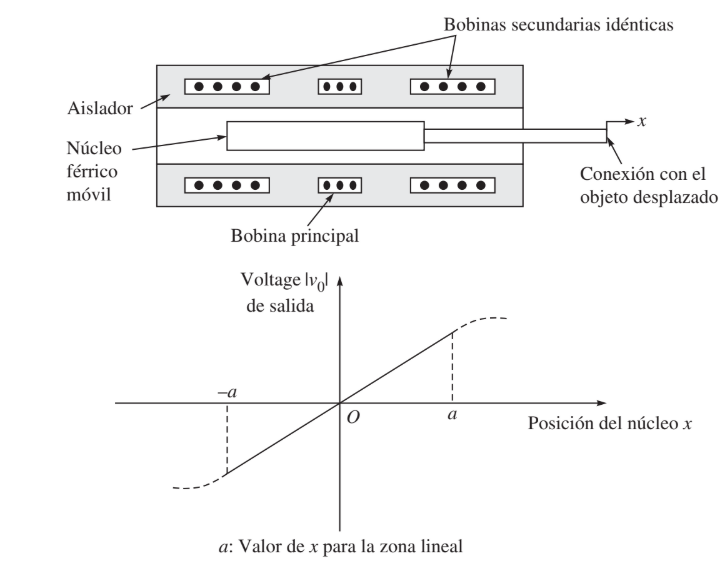
\includegraphics[width=0.700\textwidth]{img/lvdt.png}
		\caption{Esquema de funcionamiento de un LVDT.}
		\label{fig:lvdt}
	\end{figure}
	
	
	\item \textbf{Résolver}: Los resólvers proporcionan señales análogas como salida. Éstos consisten en un eje (flecha) giratorio (rotor) y una carcasa estacionaria (estator). Sus señales tienen que convertirse a la forma digital por medio de un convertidor analógico a digital antes de que la señal sea introducida a la computadora.Su funcionamiento se basa en la conversión de la posición angular del rotor en señales eléctricas proporcionales al ángulo de giro.
	
	Los resolvers se utilizan para medir el ángulo de un eje en aplicaciones donde los encoders no son viables debido a condiciones extremas como temperatura, vibraciones o interferencias electromagnéticas. Funcionan aplicando una señal de referencia de corriente alterna (CA) al rotor, lo que induce tensiones en las bobinas del estator dispuestas a 90° entre sí. Estas señales de salida tienen amplitudes proporcionales al seno y coseno del ángulo del rotor, lo que permite determinar la posición angular con alta precisión.
	\begin{figure}[h]
		\centering
		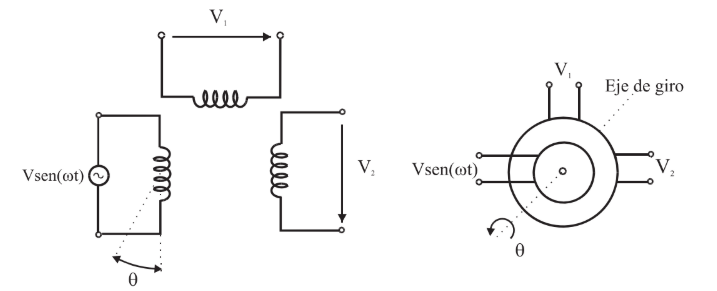
\includegraphics[width=\textwidth]{img/resolver.png}
		\caption{Esquema de funcionamiento de un resolver.}
	\end{figure}
	
	
	La imagen Figura 5 muestra el esquema de funcionamiento de un resolver, un sensor electromecánico utilizado para medir la posición angular de un eje. En el diagrama se observa un rotor, que es la parte móvil del dispositivo y está conectado al eje de giro, y un estator, que es la parte fija y contiene dos bobinas ubicadas en cuadratura, es decir, dispuestas a 90° entre sí. La señal de referencia, representada como V\( _{\text{sen}}(\omega t) \), se aplica a la bobina del rotor, lo que genera un acoplamiento electromagnético con las bobinas del estator. Este acoplamiento hace que las bobinas del estator induzcan voltajes proporcionales al ángulo $\theta$ del rotor.
	Las ecuaciones que describen el comportamiento del resolver son:
	
	\begin{equation}
		V_1 = V \sin(\omega t) \sin(\theta)
	\end{equation}
	
	\begin{equation}
		V_2 = V \sin(\omega t) \cos(\theta)
	\end{equation}
	
	Esto significa que la señal de salida en el estator depende del seno y el coseno del ángulo de giro del rotor, lo que permite calcular con precisión su posición angular mediante la relación entre ambas tensiones.  
	
\end{itemize}

\subsection{Sensores de Velocidad}
La captación de la velocidad se hace necesaria para mejorar el comportamiento dinámico de
los actuadores del robot. La velocidad de movimiento de cada actuador (que tras el reductores la velocidad de la articulación) se realimenta normalmente a un bucle de control analógico implementado en el propio accionador del elemento motor. No obstante, en ocasiones en las que el sistema de control del robot lo exija, la velocidad de giro de cada actuador es llevada hasta la unidad de control del robot.

Los sensores de velocidad incluyen:

\begin{itemize}
	\item \textbf{Todos los sensores de posición}
	\item \textbf{Tacómetro}: Estos sensores pueden encontrar directamente la velocidad en cualquier momento y sin mucha carga computacional. Éstos miden la velocidad de rotación de un elemento. Hay varios tipos de tacómetros en uso, pero un diseño sencillo se basa en la regla de Fleming, que declara que “el voltaje producido es proporcional al índice del acoplamiento inductivo”. Aquí un conductor (básicamente una bobina) se sujeta al elemento rotativo que gira en un campo magnético (estator). Conforme incrementa la velocidad del eje, el voltaje producido en las terminales de las bobinas también aumenta. De otra manera, como se muestra en la figura 6, puede colocarse un imán sobre el eje rotativo y una bobina sobre el estator. El voltaje producido es proporcional a la velocidad de rotación del eje. Esta información se digitaliza mediante un convertidor analógico-digital y se introduce en la computadora.
	\begin{figure}[h]
		\centering
		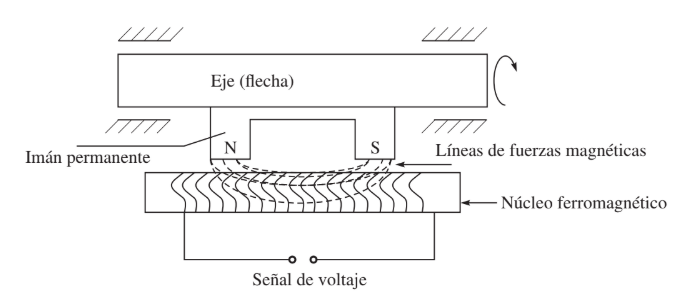
\includegraphics[width=\textwidth]{img/Diagramatacometro.png}
		\caption{Diagrama Tacómetro}
	\end{figure}
	
	
	\item \textbf{Sensor de efecto Hall}: El  principio de este sensor es el siguiente: Si una pieza plana de material conductivo llamada chip Hall se sujeta a una diferencia de potencial en sus dos lados opuestos como se indica en la figura 7, entonces el voltaje que se genera a través de las caras perpendiculares es cero. Pero si un campo magnético se induce en ángulos rectos al conductor, el voltaje se genera en las otras dos caras perpendiculares. Entre más alto sea el valor de campo, más lo será el nivel de voltaje. Si se utiliza un imán anular, el voltaje producido será proporcional a la velocidad de rotación del imán. 
	\begin{figure}[h]
		\centering
		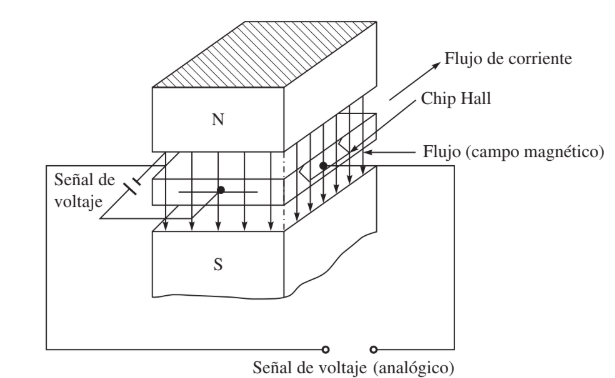
\includegraphics[width=\textwidth]{img/sensorhall.png}
		\caption{Sensor Hall}
	\end{figure}
	
\end{itemize}

\subsection{Sensores de Aceleración}
La aceleración puede obtenerse a partir de los sensores de velocidad o calculando el cambio en la posición, pero este método es ineficiente y sobrecarga la computadora, afectando el rendimiento del sistema. Una alternativa es medirla mediante la fuerza, aplicando la fórmula masa por aceleración. 
Las fuerzas se miden usando la fórmula de las galgas extensométricas, mediante la relación \( F = \frac{\Delta RAE}{RC} \) y dividiéndola por la masa del objeto obtenemos la formula de la aceleración: \[a = \frac{\Delta R A E}{R C m} \]. Donde: \begin{itemize}
	\item $F$: fuerza
	\item $\Delta R$: cambio de resistencia de la galga
	\item $A$: área
	\item $E$: módulo de elasticidad del material de la galga
	\item $R$: resistencia original de la galga
	\item $C$: constante de deformación de la galga
\end{itemize}
Este método es preferible, ya que evita la amplificación del ruido que ocurre al calcular la aceleración desde la velocidad, donde se requiere diferenciación. En cambio, la integración de la fuerza ayuda a suprimir el ruido en la señal.
Los sensores de aceleración incluyen:
\begin{itemize}
	\item \textbf{Todos los sensores de fuerza}
\end{itemize}
\subsection{Sensores de Fuerza}	
\begin{itemize}
	\item \textbf{Galgas extensométricas}: Este sensor interno tiene como principio que: “el alargamiento de un conductor aumenta su resistencia eléctrica”, debido a 2 razones principales:
	
	-	Incremento de la longitud del conductor.
	
	-	Decremento en el área del conductor.
	
	
	
	De esta forma, se pueden detectar las variaciones, ya que una resistencia normal para galgas es de 50 a 100 ohmios.
	
	Cuando el objeto al que está adherida la galga se deforma (por tensión o compresión), la longitud y la sección transversal del material de la galga cambian, lo que modifica su resistencia eléctrica. Esta variación de resistencia se mide con un circuito en puente de Wheatstone y se convierte en una señal eléctrica proporcional a la deformación.
	\begin{figure}[h]
		\centering
		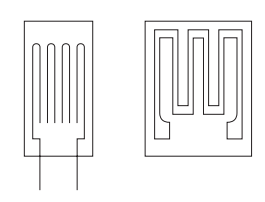
\includegraphics[width=0.5\textwidth]{img/galgas.png}
		\caption{Galgas extensométricas}
	\end{figure}
	
	\item \textbf{Interruptores de efecto Hall}: Los interruptores de efecto Hall son sensores electrónicos que detectan la presencia de un campo magnético y generan una señal de salida en respuesta.
	
	Cuando un material conductor o semiconductor, como el silicio, se somete a un campo magnético perpendicular a la dirección de la corriente que circula a través de él, se genera una diferencia de potencial (voltaje Hall) en dirección perpendicular a ambos.
	
	Los interruptores de efecto Hall utilizan este principio para detectar campos magnéticos y generar una señal de encendido o apagado.
	\begin{figure}[h]
		\centering
		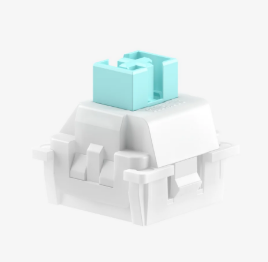
\includegraphics[width=0.5\textwidth]{img/interruptorhall.png}
		\caption{Interruptor de efecto Hall}
	\end{figure}
	
	
	\item \textbf{Interruptores piezoeléctricos}: Este sub tipo de sensor interno de fuerza utiliza el principio del efecto piezoeléctrico, el cual señala que: “cuando cristales elásticos asimétricos se deforman mediante una fuerza, se desarrollará un potencial eléctrico dentro de la red cristalina deformada”.
	
	Cuando se aplica una presión sobre la superficie del interruptor, el material piezoeléctrico dentro del dispositivo genera una pequeña carga eléctrica. Esta señal es procesada y utilizada para activar o desactivar un circuito, funcionando como un interruptor táctil sin desgaste mecánico.
	\begin{figure}[h]
		\centering
		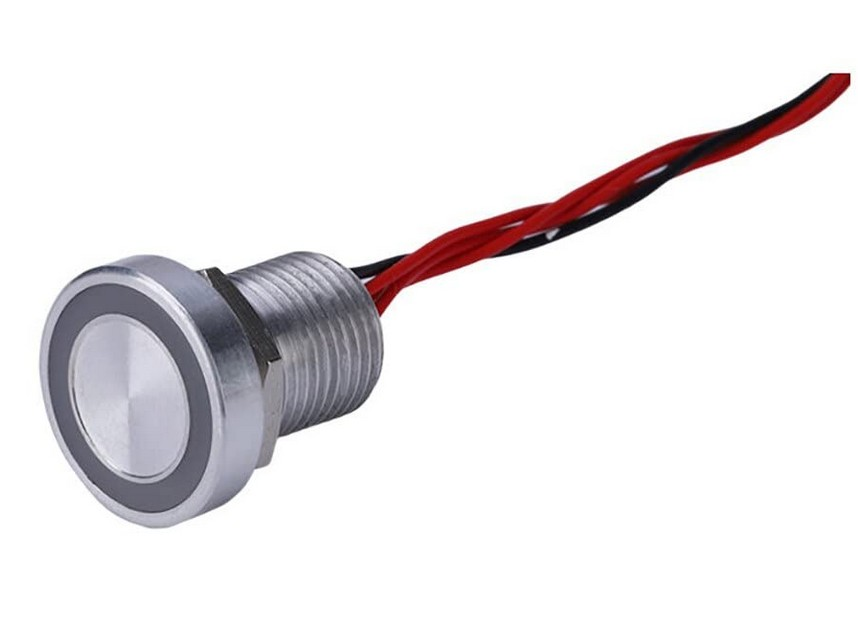
\includegraphics[width=0.5\textwidth]{img/piezoelectric-switch.jpg}
		\caption{Interruptor piezoeeléctrico}
	\end{figure}
	
\end{itemize}
